\setTopic{Sets and Functions}
\setAuthor{M. Andrew Moshier}
\setDate{October 2014}
\setCourse{Discrete Mathematics}

\setOverview{
The mathematical universe consists of various things: numbers, functions, graphs, lists and so on.
A \noexpand\emph{set} is a collection of things. 
For example, the collection of all natural numbers is a set.
A \noexpand\emph{function} is a correlation of the members of one set with members of another set.
These two abstract concepts (sets and functions) form a conceptual framework in which virtually all of mathematics can be built.
So an understanding of sets and functions is key to a rigorous approach to most other parts of mathematics.
This conceptual framework can itself be put on a formal, precise footing called the Category of Sets and Functions.

In these lectures, we build up the Category of Sets and Functions, so that we can use these things as the basic building blocks of everything else we do.
}

\chapter{Sets}

\begin{goals}
\noindent\textbf{Lecture}
\begin{itemize}
\item Describe informally the category of sets.
\item Define list set notation.
\item Introduce the idea of a subset.
\item Introduce the axiom of extensionality for sets and some of its consequences.
\end{itemize}

\noindent\textbf{Study}
\begin{itemize}
\item Demonstrate ability to determine equality of sets.
\item Develop facility in basic set theoretic notation.
\end{itemize}
\end{goals}

\section*{Introduction}

\emph{Sets} are the mathematician's way of thinking about \emph{collections} of objects. Examples will be the set of natural numbers, the set of pairs of natural numbers, the set of lists of natural numbers, and so on.
\emph{Functions} are the mathematicians way of thinking about operations, such as successor, addition, summation, and so on.

Mathematicians also use functions to model attributes of the things in a collection, like ``the color of'', ``the mass of'', ``the location of'', ``the father of'', ``the favorite book of the person to the left of'' and so on.
There is little sense in saying these are ``operations'', but they have a similar behavior. For each potential
object $x$ of the right sort (a wooden building block, for example), \emph{the color of $x$} is a specific color. Similarly,
any specific natural number $n$, ``the successor of $n$'' is another specific natural number. So ``the color of'' is a function
from the set of wooden bulding blocks to the set of colors; ``the successor of''
is a function from the set of natural numbers to set of natural numbers. Likewise, addition constitutes a function from the set of 
pairs of natural numbers to the set of natural numbers. In English we might say ``the sum of $m$ and $n$'', but we usually write $m+n$. 
Either way, any pair of natural numbers has a sum. So ``the sum of'' is an attribute of pairs of natural numbers, just like ``the color of'' is an attribute of wooden building blocks.

Taken together, sets and functions constitute a fundamental structure in contemporary mathematics called the \emph{Category of Sets and Functions}. 
This is a slight lie.
Actually, there are many different categories of sets that differ in subtle ways. 
But for most mathematics, the differences are irrelevant.
So in practice, it is safe to talk as if there is just one category of sets.
The Category of Sets and Functions sometimes abbreviated as \textbf{Set}.

To understand sets and functions as they are used in every day mathematics, we need to answer some questions:
\begin{itemize}
	\item What do we mean by saying that a set is a collection?
	\item What do we mean by saying that two sets are equal?
	\item What do we mean by saying that a function behaves like an attribute?
	\item What do we mean by saying that two functions are equal?
\end{itemize}
The answers to these leads to some basic principles for reasoning about sets and functions. 
In addition, we ways to construct sets and functions with specific behaviors. 
These lead to further principles of set and function construction.

\section*{Sets}

A set is a collection of things that are ``in'' the set. All other things are ``not in'' the set. 
For example, later we will see that the natural numbers constitute a set $\NN$. 
So $0$ is in $\NN$, $1$ is in $\NN$, and so on, but $\frac{1}2$ is not in $\NN$.
We make this precise and introduce notation for the idea.

\begin{signature}\label{sig:SetSignature}
  A \emph{set} is a mathematical entity $A$ with the following feature. 
  For any thing $x$, either $x$ \emph{is in} $A$ or $x$ \emph{is not in} $A$. 
  We write $x\in A$ if $x$ is in $A$ and $x\notin A$ if $x$ is not in $A$.

The symbol $\in$ is used in mathematics exclusively to indicate membership in a set. 
You will not see it used in any other way.  

For variety, all of the following phrases mean the same thing:
\begin{itemize}
\item $x$ is in $A$
\item $x$ is an \emph{element of} $A$
\item $x$  is a \emph{member of} $A$
\item $A$ \emph{contains} $x$
\item $x$ \emph{belongs to} $A$
\end{itemize}
\end{signature}

Basic Vocabulary \ref{sig:SetSignature} describes how we can talk about sets and elements, and how to use the notation of membership, but does not tell us that any sets actually exist. 
We will remedy that in the next sections.
Our first remedy is to make room for finite sets.

\begin{axiom}[Finite Sets] For any list $L  = [a_0,\ldots, a_{n-1}]$, there is a set, denoted by $\{a_0,\ldots,a_{n-1}\}$, so
  that $x\in \{a_0,\ldots, a_{n-1}\}$ if and only if $x=a_i$ for some
  $i<n$.  More precisely,
  \begin{itemize}
  \item $x\notin \{\}$ for any $x$ (so $\{\}$ is said to be \emph{empty});
  \item $x\in \{a_0,\ldots,a_n\}$ if and only if $x=a_0$ or $x\in
    \{a_1,\ldots,a_n\}$.
  \end{itemize}
\end{axiom}

\begin{example}
Here are some examples of sets built from finite lists:
\begin{itemize}
\item $\{\}$ -- an empty set;
\item $\{1,2,5\}$ -- a set consisting of three elements;
\item $\{\{\}\}$ -- a set consisting of one element, which is $\{\}$;
\item $\{1,2,4,\{1,2\}\}$ -- a set consisting of four elements, $1$,
  $2$, $4$ and the set $\{1,2\}$.
\item $\{4,5, \{\}, [\,]\}$ -- a set consisting of four elements. Note that
the set $\{\}$ and the list $[\,]$ are not the same things.
\item $\{1,2,3,4,3,2,1\}$ -- a set consisting of four elements, listing an element twice is redundant.
\end{itemize}
\end{example}

The study of finite sets is surprisingly complex, and comprises a large part of
the branch of mathematics called \emph{combinatorics}. We will touch on some basics
of combinatorics later in the course. 

\printbreak

\begin{exercises}
	\begin{enumerate}
  \item Let $A = \{1,\{2,3\},4\}$. Determine which of the following assertions are true.
    \begin{enumerate}
    \item $1\in A$
    \item $2\in A$
    \item $\{\}\in A$
    \item $\{2,3\}\in A$
    \item $A\in A$
    \end{enumerate}
  \item In the following examples of sets with elements following a pattern, write an expression for the same set
  that makes the pattern clearer.
  \begin{enumerate}
  \item $\{0,2,4,\ldots, 100\}$
  \item $\{1,2,4,8,\ldots, 256\}$
  \item $\{0,1,3, 6, 10,\ldots, 55\}$
  \end{enumerate}
  \end{enumerate}
\end{exercises}

\section*{Subsets}

Sets are meant to be bare collections. For a set $A$, some things are in $A$, some are not. And that's all we can say.
Unlike a list, a set has no ``initial'' element of a set.
For example, the set $\{1,2,3\}$ should be the same as the set $\{2,3,1\}$, because both have the same elements. This is an important difference between
lists and sets: $[1,2,3]$ and $[2,3,1]$ are \emph{not} the same lists because order matters in lists. 
To make this precise, we need to be clear about when sets are equal. To do this, we introduce an important definition.

\begin{defn}
  For sets $A$ and $B$, we say that \emph{$A$ is a subset of $B$} provided that every element of $A$ is an element of $B$. We also
  write this as $A\subseteq B$, and say that \emph{$A$ is included in $B$}.  We may also write $B\supseteq A$ 
  to mean the same thing, and say that \emph{$B$ is a superset of $A$}.

  If $A$ is \emph{not} a subset of $B$, we write $A\not\subseteq B$. If $A\subseteq B$ and $B\not\subseteq A$, then $A$ is called a
  \emph{proper subset of $B$}. To indicate that $A$ is a \emph{proper} subset of $B$, we may write $A\subsetneq B$.
\end{defn}

Saying $A\subseteq B$ is exactly the same as saying that for any $x$, if $x\in A$ then $x\in B$.

\begin{example}
  Here are some examples and counter-examples of the subset relation.
  \begin{itemize}
  \item $\{1,2,3\}\subseteq \{0,1,2,3\}$
  \item $\{\}\subseteq \{0\}$
  \item $A\subseteq A$ for any set $A$ because, trivially, every
    element of $A$ is an element of $A$
  \item $\{\} \subseteq A$ for any set $A$ because every element of
    $\{\}$ (there are none) is an element of $A$
  \item $\{1,2,3\}\not\subseteq \{0,2,3\}$ because $1\in \{1,2,3\}$
    but $1\notin \{0,2,3\}$
  \item $\{1,2,3\}\subseteq \{2,3,1\}$
  \end{itemize}
\end{example}

\ipadbreak

\begin{exercises}
	For each of the following pairs of sets, determine whether or
  not the first is a subset of the second. Explain your answer.
  \begin{enumerate}
  \item $\{0,1\}$ and $\{1,0\}$
  \item $\{a,b,c,d\}$ and $\{a,b,d,e,c\}$
  \item $\{\}$ and $\{\{\}\}$
  \item $\{0,3,6,10\}$ and $\{10,9,8,7,6,5,4,2,1, 0\}$
  \end{enumerate}
\end{exercises}

\section*{Equal Sets}

We can summarize two
useful properties of $\subseteq$ as follows.
\begin{itemize}
	\item{}[Reflexivity]  For any set $A$, $A \subseteq A$. We say $\subseteq$ is \emph{reflexive}.
	\item{}[Transitivity] For any sets $A$, $B$ and $C$,
	if $A\subseteq B$ and $B\subseteq C$, then $A\subseteq C$. We say $\subseteq$ is \emph{transitive}.
\end{itemize}
Another familiar example of a reflexive, transitive
relation is $\leq$ on the natural numbers. In fact there are many examples of reflexive transitive relations throughout mathematics. 

The relation $\leq$ is also \emph{anti-symmetric}, meaning that if $m\leq n$ and $n\leq m$ then $m=n$. 
Suppose $A\subseteq B$ and $B\subseteq A$. Then, by definition $A$ and $B$ have the exact same elements.  By our understanding of sets as collections,
$A$ and $B$ must be equal. So we state this as another axiom.

\begin{axiom}\label{ax:set-extensionality}
[\textbf{The Axiom of Set Extensionality}]
For sets $A$ and $B$, if $A\subseteq B$ and $B\subseteq A$, then $A=B$. In other words, $\subseteq$ is anti-symmetric.
\end{axiom}

Based on this, we can already establish a useful fact: there is exactly one empty set. To set the tone for what follows, we make this a formal claim.

\begin{lemma}
	There is exacty one empty set.
\begin{proof}
	We have already noted that the set built from an empty list $\{\,\}$ has no elements. So there is at least one empty set.
	
	Suppose $E$ is a set with no elements. Then $E\subseteq \{\,\}$ because every element of $E$ (there are none) is an element of $\{\,\}$. Similarly, $\{\,\}\subseteq E$ because every element of $\{\,\}$ (again, there are none) is an elemen of $E$. So by Axiom~\ref{ax:set-extensionality} $E = \{\,\}$.
\end{proof}
\end{lemma}

\begin{defn}
  The set $\{\}$ is also denoted by $\emptyset$. This is a universally accepted symbol for the empty set.
\end{defn}

Set extensionality makes precise the idea that a set by itself does
not have any structure other than what members it possesses.
To emphasize this, sometimes it is useful to
depict a set with elements scattered about something like \usetikzlibrary{fit,shapes}
\[\begin{tikzpicture}[ >=stealth, bullet/.style={ fill=black, circle,
    minimum width=1pt, inner sep=2pt }, projection/.style={ ->, thick,
    shorten <=2pt, shorten >=2pt }, every fit/.style={ ellipse, draw,
    inner sep=2pt } ]
  \foreach \x/\y/\l in {0.4/1/d,-0.2/2/c/,0/3/b,0.5/4/a}
  \node[bullet,label=left:$\l$] (a\y) at (\y,\x) {};
  \node[draw,fit=(a1) (a2) (a3) (a4),minimum width=2cm] {} ;
\end{tikzpicture}
\]
with the elements scattered about. Evidently, a re-arrangement of the
elements does not change the depicted set. So
\[\usetikzlibrary{fit,shapes}
\begin{tikzpicture}[ >=stealth, bullet/.style={ fill=black, circle,
    minimum width=1pt, inner sep=2pt }, projection/.style={ ->, thick,
    shorten <=2pt, shorten >=2pt }, every fit/.style={ ellipse, draw,
    inner sep=2pt } ]
  \foreach \x/\y/\l in {0.3/2/d,-0.2/3/c/,0/4/b,-0.5/1/a}
  \node[bullet,label=left:$\l$] (a\y) at (\y,\x) {};
  \node[draw,fit=(a1) (a2) (a3) (a4),minimum width=2cm] {} ;

\end{tikzpicture}
\]
is the same set. Depicting a subset of a set is a simple
matter of drawing a smaller boundary around some of the elements as in the following.
\[\usetikzlibrary{fit,shapes}
\begin{tikzpicture}[ >=stealth, bullet/.style={ fill=black, circle,
    minimum width=1pt, inner sep=2pt }, projection/.style={ ->, thick,
    shorten <=2pt, shorten >=2pt }, every fit/.style={ ellipse, draw,
    inner sep=2pt } ]
  \foreach \x/\y/\l in {0.3/2/d,-0.2/3/c/,0/4/b,-0.5/1/a}
  \node[bullet,label=left:$\l$] (a\y) at (\y,\x) {};
  \node[draw,fit=(a1) (a2) (a3) (a4),minimum width=2cm] {} ;
  \node[draw, fit = (a2) (a3), minimum width=2cm] {};
\end{tikzpicture}
\]
\ipadbreak

\begin{exercises}
Draw depictions of the following sets
  \begin{enumerate}
  \item $\{1,4,5,2,3\}$
  \item $\{1,2,3,\ldots, 23\}$
  \item $\{a,b,c,d,e\}$ and $\{c,e,f,g\}$ on the same diagram
  \item $\{a, e, b,c,e\}$ [sic]
  \item $\{1,3,6,7\}$ and $\{1,3,5,6,7,9\}$ on the same diagram
  \item $\{\bot,\top$
  \item $\{\bullet\}$
  \item $\{\top,\bot,3,5,1, \bullet\}$
  \end{enumerate}
\end{exercises}

\chapter{Functions}

\begin{goals}
\noindent\textbf{Lecture}
\begin{itemize}
\item Introduce basic structure of functions
\item Define the identity functions and function composition
\item Introduce internal diagrams of functions.
\end{itemize}

\noindent\textbf{Study}
\begin{itemize}
\item Be able to determine equality of functions
\item Use internal diagrams to depict function composition
\end{itemize}
\end{goals}

\emph{Functions}
(perhaps in your calculus courses) are often talked about as \emph{operations}. 
For example, \[f(x) = x^2-1\]
can be seen as an operation that transforms a number $x$ into its
square. But it can also be seen as an attribute (the ``square of
$x$''). The ``operational'' view is informal, and often useful. As we will see,
though, it gets an important aspect of functions wrong because
two entirely different operations may define the same function.

Informally, a function ``takes'' an argument from a given set as input and ``produces'' an output in a given set.
So the function $f$ defined by $f(x)=x^2 + 2x + 1$ might ``take'' the natural number $2$
and ``produce'' the natural number $10$. That is, $f(3)=3^2 + 1 = 10$. 
We begin by introducing the vocabulary of functions.

\begin{signature}
	\begin{itemize}
	\item For a set $A$ and a set $B$, there are some things called 
	\emph{functions from $A$ to $B$}, with a function $f$ from $A$ to $B$ 
	being writing $\fromto fAB$ or $A\stackrel{f}{\to} B$. 
	
	\item For $\fromto fAB$, the set $A$ is called the \emph{domain} of $f$
	and $B$ is called the \emph{codomain} of $f$.
	
	\item For any function $\fromto fAB$ and every element $a\in A$, $f$ and $a$ determine an element of $B$,
	written $f(a)$, and read ``$f$ of $a$''.
	\end{itemize}
\end{signature}

Often, a function $\fromto fAB$ is \emph{defined} by a rule, just as your are familiar in other parts of mathematics. There are two fundamental (trivial) types of rules that can be used to build functions.

\begin{axiom}
	\begin{itemize}
		\item For any set $A$, there is a function $\fromto {\id_A}AA$ defined by the rule $\id_A(x)=x$. This is called the \emph{identity} function on $A$
		\item For any two functions $\fromto fAB$ and $\fromto gBC$, there is a function $\fromto {g\circ f}AC$ defined by the rule $(g\circ f)(x)=g(f(x))$.
		      This is called the composition of $g$ and $f$ (or sometimes ``$g$ following $f$'').
	\end{itemize}
\end{axiom}

Other words for function are \emph{map}, \emph{transformation} and \emph{operation}.
We will discuss, however, why ``operation'' can be misleading.

Notice that $g\circ f$ is only defined when the \emph{domain} of $g$ matches the codomain of $f$. Also, be careful about definitions like $f(x)=1/x$. This does not define a function on the real numbers because $f(0)$ is undefined. In other words, to be a function, $f$ must determine an element of the codomain for each element of the domain.

To depict a function on small sets, we can use the simple internal diagrams of the last section. For example,
\[
  \begin{tikzpicture}[
    >=stealth,
    bullet/.style={
      fill=black,
      circle,
      minimum width=1pt,
      inner sep=1pt
    },
    projection/.style={
      ->,
      thick,
      shorten <=2pt,
      shorten >=2pt
    },
    every fit/.style={
      ellipse,
      draw,
      inner sep=0pt
    }
  ]
    \foreach \x/\y/\l in {0.4/1/d,-0.2/2/c/,0/3/b,0.5/4/a}
      \node[bullet,label=left:$\l$] (a\y) at (\x,\y) {};

    \foreach \x/\y/\l in {4.1/1/4,3.2/2/3,4.3/3/2,4/4/1}
      \node[bullet,label=right:$\l$] (b\y) at (\x,\y) {};

    \node[draw,fit=(a1) (a2) (a3) (a4),minimum width=2cm] {} ;
    \node[draw,fit=(b1) (b2) (b3) (b4),minimum width=2cm] {} ;

    \draw[projection] (a1) -- (b4);
    \draw[projection] (a2) -- (b2);
    \draw[projection] (a3) -- (b1);
    \draw[projection] (a4) -- (b3);
  \end{tikzpicture}
\]
depicts a function from the set $\{a,b,c,d\}$ to the set $\{1,2,3,4\}$.

  Composition can be illustrated using internal diagrams. For example,
  \[
    \begin{tikzpicture}[
      >=stealth,
      bullet/.style={
        fill=black,
        circle,
        minimum width=1pt,
        inner sep=1pt
      },
      projection/.style={
        ->,
        thick,
        shorten <=2pt,
        shorten >=2pt
      },
      projectionC/.style={
        ->,
        thick,
        dashed,
        shorten <=2pt,
        shorten >=2pt
      },
      every fit/.style={
        ellipse,
        draw,
        inner sep=0pt
      }
    ]
      \foreach \x/\y/\l in {0.4/1/d,-0.2/2/c/,0/3/b,0.5/4/a}
        \node[bullet,label=left:$\l$] (a\y) at (\x,\y) {};

      \foreach \x/\y/\l in {3.5/2/4,4.1/3/3,3.2/4/2,4/5/1}
        \node[bullet,label=below:$\l$] (b\y) at (\x,\y) {};

      \foreach \x/\y/\l in {7.8/1/u,8.2/2/v,7.3/3/w,7.9/4/x, 8.0/5/z}
        \node[bullet,label=right:$\l$] (c\y) at (\x,\y) {};

      \node[blue] at (2,5) {$f$};
      \node[green] at (6,5.5) {$g$};
      \node[red] at (4,0.5) {$g\circ f$};

      \node[draw,fit=(a1) (a2) (a3) (a4),minimum width=2cm] {} ;
      \node[draw,fit=(b2) (b3) (b4) (b5),minimum width=2cm] {} ;
      \node[draw,fit=(c1) (c2) (c3) (c5),minimum width=2cm] {} ;

      \draw[projection,blue] (a1) -- (b2);
      \draw[projection,blue] (a2) -- (b2);
      \draw[projection,blue] (a3) -- (b3);
      \draw[projection,blue] (a4) -- (b5);
      \draw[projection,green] (b2) -- (c1);
      \draw[projection,green] (b3) -- (c2);
      \draw[projection,green] (b4) -- (c3);
      \draw[projection,green] (b5) -- (c5);
      \draw[projectionC,red] (a1) -- (c1);
      \draw[projectionC,red] (a2) -- (c1);
      \draw[projectionC,red] (a3) -- (c2);
      \draw[projectionC,red] (a4) -- (c5);
    \end{tikzpicture}
	\]
	
\begin{exercises}
	Use internal diagrams for the following exercises.
	\begin{enumerate}
		\item Depict four different functions from the set $\{1,2,3\}$ to the set $\{\bot,\top\}$. [Draw four different diagrams.]
		\item Depict all of the functions from $\{\bullet\}$ to $\{a,b,c\}$
		\item Depict all of the functions from $\{a,b,c\}$ to $\{\bullet\}$
		\item Are there any functions from $\{a,b\}$ to $\emptyset$?
		\item Are there any functions from $\emptyset$ to $\{a,b\}$? If there are, how many?
		\item For each of the following diagrams, determine whether or not the
  diagram depicts a function. If not, explain why not.
  \begin{multicols}{2}
    \begin{enumerate}
    \item
      \begin{tikzpicture}[ scale=.75, >=stealth, bullet/.style={
          fill=black, circle, minimum width=1pt, inner sep=1pt },
        projection/.style={ ->, thick, shorten <=2pt, shorten >=2pt },
        every fit/.style={ ellipse, draw, inner sep=0pt } ]
        \foreach \x/\y/\l in {0.4/1/d,-0.2/2/c/,0/3/b,0.5/4/a}
        \node[bullet,label=left:$\l$] (a\y) at (\x,\y) {};

        \foreach \x/\y/\l in {4.1/1/4,3.2/2/3,4.3/3/2,4/4/1}
        \node[bullet,label=right:$\l$] (b\y) at (\x,\y) {};

        \node[draw,fit=(a1) (a2) (a3) (a4),minimum width=2cm] {} ;
        \node[draw,fit=(b1) (b2) (b3) (b4),minimum width=2cm] {} ;

        \draw[projection] (a1) -- (b4); \draw[projection] (a2) --
        (b3); \draw[projection] (a3) -- (b1); \draw[projection] (a4)
        -- (b3);
      \end{tikzpicture}
    \item \begin{tikzpicture}[ scale=.75, >=stealth, bullet/.style={
          fill=black, circle, minimum width=1pt, inner sep=1pt },
        projection/.style={ ->, thick, shorten <=2pt, shorten >=2pt },
        every fit/.style={ ellipse, draw, inner sep=0pt } ] \foreach
        \x/\y/\l in {0.4/1/d,-0.2/2/c/,0/3/b,0.5/4/a}
        \node[bullet,label=left:$\l$] (a\y) at (\x,\y) {};

        \foreach \x/\y/\l in {4.1/1/4,3.2/2/3,4.3/3/2,4/4/1}
        \node[bullet,label=right:$\l$] (b\y) at (\x,\y) {};

        \node[draw,fit=(a1) (a2) (a3) (a4),minimum width=2cm] {} ;
        \node[draw,fit=(b1) (b2) (b3) (b4),minimum width=2cm] {} ;

        \draw[projection] (a1) -- (b4); \draw[projection] (a2) --
        (b3); \draw[projection] (a3) -- (b1); \draw[projection] (a4)
        -- (b3); \draw[projection] (a2) -- (b2);
      \end{tikzpicture}
    \item \begin{tikzpicture}[ scale=.75, >=stealth, bullet/.style={
          fill=black, circle, minimum width=1pt, inner sep=1pt },
        projection/.style={ ->, thick, shorten <=2pt, shorten >=2pt },
        every fit/.style={ ellipse, draw, inner sep=0pt } ] \foreach
        \x/\y/\l in {0.4/1/d,-0.2/2/c/,0/3/b,0.5/4/a}
        \node[bullet,label=left:$\l$] (a\y) at (\x,\y) {};

        \foreach \x/\y/\l in {4.1/1/4,3.2/2/3,4.3/3/2,4/4/1}
        \node[bullet,label=right:$\l$] (b\y) at (\x,\y) {};

        \node[draw,fit=(a1) (a2) (a3) (a4),minimum width=2cm] {} ;
        \node[draw,fit=(b1) (b2) (b3) (b4),minimum width=2cm] {} ;

        \draw[projection] (a1) -- (b1); \draw[projection] (a2) --
        (b1); \draw[projection] (a3) -- (b1); \draw[projection] (a4)
        -- (b1);
      \end{tikzpicture}
    \item \begin{tikzpicture}[ scale=.75, >=stealth, bullet/.style={
          fill=black, circle, minimum width=1pt, inner sep=1pt },
        projection/.style={ ->, thick, shorten <=2pt, shorten >=2pt },
        every fit/.style={ ellipse, draw, inner sep=0pt } ] \foreach
        \x/\y/\l in {0.4/1/d,-0.2/2/c/,0/3/b,0.5/4/a}
        \node[bullet,label=left:$\l$] (a\y) at (\x,\y) {};

        \foreach \x/\y/\l in {4.1/1/4,3.2/2/3,4.3/3/2,4/4/1}
        \node[bullet,label=right:$\l$] (b\y) at (\x,\y) {};

        \node[draw,fit=(a1) (a2) (a3) (a4),minimum width=2cm] {} ;
        \node[draw,fit=(b1) (b2) (b3) (b4),minimum width=2cm] {} ;

        % \draw[projection] (a1) -- (b4);
        \draw[projection] (a2) -- (b3); \draw[projection] (a3) --
        (b1); \draw[projection] (a4) -- (b3);
      \end{tikzpicture}
	  \end{enumerate}
	  \end{multicols}
		\item Let $A = \{1,2,3\}$. Let $B=\{a,b,c,e\}$ and let $C = \{\bot,\top\}$. Depict some functions $\fromto fAB$, $\fromto gBC$, and $g\circ f$. 
		\item Think about how you might depict a function $\fromto hAA$ using only one picture of the set $A$. Describe what you would do, and provide an example.  
	\end{enumerate}
\end{exercises}

\section*{Equal Functions and External Diagrams}

Just like sets, we need a way to say when two functions are equal.
Let $\NN$ denote the set of natural numbers. 
Then define $\fromto f\NN\NN$ by the rule
\[f(n) = n^2 +  2n + 1.\]
Likewise, define $\fromto g\NN\NN$ by the rule
\[g(n) = (n+1)^2.\]
Evidently, for each $n\in\NN$, it is true that $f(n) = g(n)$. So even though $f$ and $g$ are defined by different
\emph{operations}, the two functions yield the same results. As with sets, this leads to
an axiom for equality of functions.

\begin{axiom}[\textbf{The Axiom of Function Extensionality}]
	For functions $\fromto fAB$ and $\fromto gAB$, if it is the case that $f(x)=g(x)$ for all $x\in A$, then $f=g$.
	Note that equality of functions only makes sense when the two functions share the same domain and the same codomain.
\end{axiom}

If we not concerned about the detailed internals sets, but only with
how functions interact, then function can be depicted very simply as $A
\stackrel{f}{\longrightarrow} B$. So a composition of functions can be
depicted as in
\[
\tikzset{>=stealth}
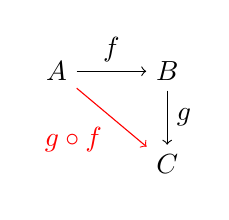
\begin{tikzpicture}[every node/.style={midway}]
\matrix[column sep={4em,between origins},
        row sep={2em}] at (0,0)
{ \node(A)   {$A$}  ; & \node(B) {$B$}; \\
                      & \node(C) {$C$}; \\};
\draw[->] (A) -- (B) node[anchor=south]  {$f$};
\draw[->] (B) -- (C) node[anchor=west]  {$g$};
\draw[->,red] (A) -- (C) node[anchor=north east] {$g\circ f$};
\end{tikzpicture}
\]
We do not really need to draw $g\circ f$ as a separate arrow because 
the \emph{path} from $A$ to $B$ to $C$ is already implicitly a depiction of $g\circ f$. So the simpler diagram 
\[
\tikzset{>=stealth}
\begin{tikzpicture}[every node/.style={midway}]
\matrix[column sep={4em,between origins},
        row sep={2em}] at (0,0)
{ \node(A)   {$A$}  ; & \node(B) {$B$}; \\
                      & \node(C) {$C$}; \\};
\draw[->] (A) -- (B) node[anchor=south]  {$f$};
\draw[->] (B) -- (C) node[anchor=west]  {$g$};
\end{tikzpicture}
\]
shows the same information, namely, that $\fromto fAB$ and $\fromto gBC$ are functions and therefore, $g\circ f$ is too.

Now a diagram such as this
\[
\tikzset{>=stealth}
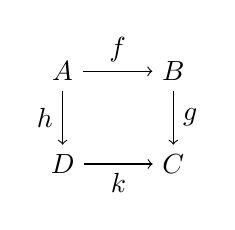
\begin{tikzpicture}[every node/.style={midway}]
\matrix[column sep={4em,between origins},
        row sep={2em}] at (0,0)
{ \node(A)   {$A$}  ; & \node(B) {$B$}; \\
  \node(D)   {$D$}  ; & \node(C) {$C$}; \\};
\draw[->] (A) -- (B) node[anchor=south]  {$f$};
\draw[->] (B) -- (C) node[anchor=west]  {$g$};
\draw[->] (A) -- (D) node[anchor=east] {$h$};
\draw[->] (D) -- (C) node[anchor=north] {$k$};
\end{tikzpicture}
\]
depicts two composite functions $g\circ f$ and $k\circ h$, but $g\circ f$ and $k\circ k$ may not be equal.
We say that
the diagram \emph{commutes} or that it is a \emph{commutative diagram}
if $g\circ f = k\circ h$. In other words, saying that a certain diagram commutes \emph{is} an assertion that certain functions are equal.


\begin{exercises}
\begin{enumerate}
\item  For each of the following pairs of functions $\NN\to\NN$, determine whether they are equal and explain why or why not.
  \begin{enumerate}
  \item $f(n) = 2n + 3$ and $g(m) = 2m + 3$
  \item $f(n) = 2^{n+1} - 1$ and $g(n) = \sum_{i=0}^n2^i$
  \item $f(n) =  n^2 + 5n + 6$ and $g(n) = (n+3)(n+2)$
  \item $f(n) = n^4 - 10n^3 + 35n^2 + 50n + 24$ and $g(n) = 24$
  \end{enumerate}
\item Let $\RR$ denote the set of all real numbers. Let $f(x) = \tan(x)$. Explain why this does \emph{not} define a function from $\RR$ to $\RR$.
\item Suppose the following functions exist: $\fromto fAB$, $\fromto
  gBC$, $\fromto aAD$, $\fromto bCD$.  Draw a commutative diagram
  asserting that $b\circ g\circ f = a$.
\item Suppose the following functions exist: $\fromto fCA$, $\fromto gCB$,
$\fromto hCP$, $\fromto pPA$ and $\fromto qPB$. Draw a commutative diagram
asserting that $f=p\circ h$ and $g=q\circ h$.
\end{enumerate}
\end{exercises}

\chapter{Building Sets and Functions}

\begin{goals}
	\noindent\textbf{Lecture}
	\begin{itemize}
	\item Characterize and define
		 \begin{itemize}
			 \item Pointer and constant functions
		 	\item The set of natural numbers
			\item Products of sets
			\item Exponents of sets
			\item Solution sets
			\item Characteristic functions
		 \end{itemize}
	\item Introduce the idea of a \emph{universal} construction.
	\end{itemize}

	\noindent\textbf{Study}
	\begin{itemize}
	\item Be able to calculate membership in various constructed sets 
	\item Learn to use universal constructions to define functions. 
	\end{itemize}
\end{goals}

\section{Introduction}

So far, we have been able to think mainly about finite sets and a few informally defined functions on, say, the real numbers or the natural numbers.
To fill out out understanding of sets, we need to be able to build sets for specific purposes. Two finite sets will play a particularly important role. The first, which we denote by $\One$, is  set with one element; the second, which we denote by $\Two$, is a set with two elements. It does not matter at all \emph{what} elements are in these because, as we will soon see, any two sets of the same size are interchangible. What `interchangible' means is discussed later. What `same size' means is obvious for finite sets, but not at all obvious for infinite ones. We discuss the general situation later as well.

For the time being, we merely need to agree on a fixed set with one element and a fixed set with two elements. The particular choices I make here will be clearer as we put them to use.

\begin{defn}
	Let $\bullet$, $\bot$ and $\top$ be fixed sybmols. Then define
	\begin{align*}
		\One &= \{\bullet\}\\
		\Two &= \{\bot,\top\}
	\end{align*} 
	The single element of $\One$ is intended to look like a generic point in an internal diagram. The element $\top$ is meant to remind you of the letter `T'
	(short for `True') and $\bot$ is meant to be the opposite of $\top$ (that is, 'False').
\end{defn}

Although we will not define any of the following except $\NN$ explicitly, it is useful also to have names for various sets of numbers.

\begin{defn}
	The following sets are denoted by special symbols:
	\begin{align*}
		\NN &= \text{the set of natural numbers}
		\ZZ &= \text{the set of integers}\\
		\QQ &= \text{the set of rational numbers}\\
		\RR &= \text{the set of real numbers}\\
		\CC &= \text{the set of complex numbers}
	\end{align*}
\end{defn}

\section{Elements, Pointers and Constant Functions}

Suppose we are told that $\fromto p\One A$ is a function. Since $\bullet\in\One$, this function determines 
an element of $A$, namely $p(\bullet)$. A picture of the situation might be this:
\[
  \begin{tikzpicture}[
    >=stealth,
    bullet/.style={
      fill=black,
      circle,
      minimum width=1pt,
      inner sep=1pt
    },
    projection/.style={
      ->,
      thick,
      shorten <=2pt,
      shorten >=2pt
    },
    every fit/.style={
      ellipse,
      draw,
      inner sep=0pt
    }
  ]
    \node[bullet] (p) at (0,2.5) {};

    \foreach \x/\y/\l in {4.1/1/4,3.2/2/3,4.3/3/2,4/4/1}
      \node[bullet,label=right:$\l$] (a\y) at (\x,\y) {};

    \node[draw,fit=(p),minimum width=1cm, minimum height=1cm] {} ;
    \node[draw,fit=(a1) (a2) (a3) (a4),minimum width=2cm] {} ;

    \draw[projection] (p) -- (a3);
  \end{tikzpicture}
\]
Since $\One$ has only a single element, it can ``point'' only to a single element of $A$. So we might refer to a function
$\One\to A$ as a \emph{pointer} into $A$. Each pointer determines an element of $A$. And conversely, it shuold be
possible to point to any element of $A$. This leads to our first axiom guaranteeing that certain functions exist.

\begin{axiom}
	For any set $A$, and any $a\in A$, there is a pointer $\fromto {\hat a}\One A$ so that $\hat{a}(\bullet)=a$.
\end{axiom}

Looking at functions in the other direction, if $\fromto fA\One$ and $\fromto gA\One$ are functions, then $f(a)=\bullet=g(a)$
is true for every $a\in A$. So $f=g$ by extensionality. In other words, there is at most one function from $A$ to $\One$.
But the $f(x)=\bullet$ is just about as trivial a rule as possible. This leads to another axiom.

\begin{defn}
	A set $T$ is \emph{terminal} if it is the case that for any set $A$ there is exactly one function from $A$ to $T$.
\end{defn}

\begin{axiom}
	The set $\One$ is a terminal set. We denote the unique function from $A$ to $\One$ by $\fromto \diamond_A{A}\One$.
	Note that the rule defining $\diamond_A$ is 
	\[\diamond_A(x)=\bullet.\]
\end{axiom} 

Using $\diamond_A$ and $\hat{b}$ for an eleent $b\in B$, we can now define constant functions. That is $\hat{b}\circ\diamond_A$
is a function from $A$ to $B$ defined by $(\hat{b}\circ\diamond_A)(x) = \hat{b}(\diamond_A(x))= \hat{b}(\bullet) = b$, Simplifying, this is the function sending any element of $A$ to the same result ($b$). 

\begin{exercises}
	\begin{enumerate}
		\item Show that for any pointer $\fromto p\One A$, it is the case that $\widehat{p(\bullet)}=p$.
		\item Suppose that $\fromto fAB$ is a function. Show that for every $a\in A$, $\widehat{f(a)} = f\circ \hat{a}$.
		\item Show that any set with exactly one element is a terminal set. [This is the sense in which it did not matter
		how we choose the element of $\One$.]
	\end{enumerate}
\end{exercises}

\section{Solution Sets, Subsets, Characteristic Functions}

Suppose we are given two functions that are ``parallel'': $\fromto fAB$ and $\fromto gAB$. Then for some value $a\in A$,
it might be the case that $f(a)=g(a)$. We could call such a value a \emph{particular solution}. It might be the case that there are no particular solutions.
For example, there are no natural numbers $n$ such that $n+1 = n$. On the other hand, there might be many particular solutions. 
For example, let $f(x)=x^3$ and let $g(x)= 6x^2 - 11x + 6$ both as functions on the natural numbers. Then it is easy to check that $1$, $2$ and $3$ 
solve the equation. In fact, these three are the only particular solutions. We generalize
as follows.

\begin{defn} 
	For functions $\fromto fAB$ and $\fromto gAB$, a \emph{solution}
is a function $\fromto sCA$ so that $f\circ s = g\circ s$. Thus for example, if $a\in A$ is a particular
solution then the pointer $\hat a$ is a solution. 

	For functions $\fromto fAB$ and $\fromto gAB$, an \emph{equalizer} is solution $\fromto eEA$
	and so that for any solution $\fromto sCA$, there is exactly one function $\fromto hCE$ 
	so that $e\circ h = k$.
\end{defn}

\begin{axiom}
	For functions $\fromto fAB$ and $\fromto gAB$, the collection of all particular solutions to the equation $f(x)=g(x)$ form a set, denoted by
	$\{x\in A\st f(x) = g(x)\}$. Furthermore, the function $\fromto i{\{x\in A\st f(x)=g(x)\}}A$ defined by the rule $i(x) = x$ (called 
	an \emph{inclusion map}) is an equalizer for $f$ and $g$.
\end{axiom}

This axiom tells us two things. First, we can form a subset of $A$ by specifying an equation $f(x)=g(x)$
for functions $\fromto {f,g}AB$, and picking out the particular solutions. Second, a subset formed in this way
``embeds'' in the given set $A$ by its inclusion map. It would be good to know that any subset of $A$ can be described
as an equalizer of some pair of functions. This is where $\Two$ plays a role.

Suppose $c\in C$ and $\fromto fAC$ is a function, then we can form the equalizer of $f$ and the constant function
$\hat{c}\circ\diamond_A$. This is more easily written we $\{x\in A\st f(x)=c\}$. We may also abbreviate this as $f^{-1}(c)$. 

\begin{defn}
	A \emph{subset classifier} is a set $S$ with an element $t\in S$ so that for any sets $B$ and $A$
	where $B\subseteq A$, there is exactly one function $\fromto kTA$ so that $B = \{x\in A\st k(x)=t\}.$
\end{defn}

\begin{axiom}
	The set $\Two$ with the distiguished element $\top$ is a subset classifier. For subset $B\subseteq A$,
	the function corresponding to $B$, called the \emph{characteristic
	function of $B$}, is denoted by $\kappa_B$. In other words, $\kappa_B$ is the unique function
	for which $B = \{x\in A\st k(x)=\top\}$.
\end{axiom}

For $B\subseteq A$, the characteristic function is defined by the rule
\[\kappa_B(x) = \begin{cases}
	\top &\text{ if } x\in B\\
	\bot &\text{ otherwise}
\end{cases}
\]

\section{Product Sets and Functions of Two Variables}

We should be able to deal with functions, such as a function defined by the rule $f(x,y) = x+y$. To account for functions of two or more arguments, we take our cue from Descartes. He studied the plane in terms of a coordinate system consisting of the so-called $x$-axis and $y$-axis. Once we have decided where to place the axes, a pair $(2,3)$ determines 
a point on the plane, and any point in the plane $p$ determines a pair. So Descartes realized that we might as well just say that the plane actually \emph{is} the collection of 
all pairs of real numbers. What makes this work is that points in the plane \emph{project} onto the two axes. Products
of sets generalize this idea.

\begin{defn}
For sets $A$ and $B$, a \emph{table} consists of two functions $\fromto fCA$ and $gCB$. Note that the two functions
have the same domain. We may call the two functions \emph{legs}.

For sets $A$ and $B$, a \emph{product of $A$ and $B$} is a table $\fromto pPA$ and $\fromto qPB$ so that
for any table $\fromto fCA$ and $\fromto gCB$, there is exactly one function $\fromto hCP$ for which
$f = p\circ h$ and $g= q\circ h$. For a product, the functions $p$ and $q$ are called the \emph{projections}.
\end{defn}

\begin{axiom}
	For sets $A$ and $B$, the collection of all pairs $(a,b)$ where $a\in A$ and $b\in B$ is a set, denoted by $A\times B$. 
	The functions $\fromto {\pi_0}{A\times B}A$ and $\fromto {\pi_1}{A\times B}B$ defined by the rules $\pi_0(a,b)=a$
	and $\pi_1(a,b)=b$ are projections. For $\fromto fCA$ and $\fromto gCB$, the unique function required by
	the product may be denoted by $\langle f,g\rangle$.
\end{axiom}

For $\fromto fCA$ and $\fromto gCB$, the function $\fromto {\langle f,g\rangle}C{A\times B}$ is defined by 
the rule $\langle f,g\rangle(x)=(f(x),g(x))$.

Suppose we are given two unrelated functions $\fromto fAB$ and $\fromto gCD$. We can now form a single function
from $A\times C$ to $B\times D$ by combining $f$ and $g$ ``independently''. That is, define $f\times g = \langle f\circ \pi_0,g\circ \pi_1\rangle$. Calculating concretely in terms of elements $(f\times g)(x,y) = (f(x),g(y))$. 

\section{Function Sets and Partial Evaluation}

A function from $A$ to $B$ might depend on a parameter from $C$. 
For example, the function $\fromto f\RR\RR$ defined by the rule $f(x) = \sin(x + c)$ depends on the constant $c$.
There is a related function $\fromto g{\RR\times \RR}\RR$ defined by $g(c,x) = \sin(x+c)$. Evidently, $g$
describes the same behavior as $f$, but it makes the parameter explicit. This leads to the following definition.

\begin{defn}
	For sets $A$ and $B$, a \emph{parametric function from $A$ to $B$} is a function $\fromto g{C\times A}B$ for some set $C$.
	The set $C$ is the \emph{set of parameters}.
	
	Suppse $\fromto f{D\times A}B$ is a parametric function with parameter set $D$ and $\fromto kCD$ is a function.
	Then we can form another parametric function with parameters in $C$ by composition: $f\circ (k\times \id_A)$.
	In this setting, we may refer to $k$ as a \emph{change of parameters}. 
	
	An \emph{evaluation map} for $A$ and $B$ is a parameteric function $\fromto a{F\times A}B$, so that for any 
	parametric function $\fromto g{C\times A}B$ there is exactly one change of parameters $\fromto hCF$ so that
	$g = a\circ (h\times \id_A)$. In that case, $F$ is called a \emph{function set} or an \emph{exponential}.
\end{defn}

\begin{axiom}
	For sets $A$ and $B$, the collection of all functions from $A$ to $B$, denoted by $B^A$, is a set. Moreover,
	there is an evaluation map $\fromto \alpha{B^A\times A}B$ defined by the rule $\alpha(f,x) = f(x)$.
\end{axiom}

Suppose $\fromto f{C\times A}B$ is a parametric function. The axiom says that there must be a unique change of parameters
function from $C$ to $B^A$. That is, $h(c)$ must be a function from $A$ to $B$ so that $\alpha(h(c),a) = f(c,a)$
for every $c\in C$ and every $a\in A$. But $\alpha$ just evaluates a given function at a given element, so $\alpha(h(c),a)=h(c)(a)$. This tells us what $h(c)$ is. Namely, $h(c)$ is the function defined by the rule $h(c)(x) = f(c,x)$.

\section{Powersets}

The exponential $\Two^A$ for any set $A$ is the set of all characteristic maps on $A$. So the elements of $\Two^A$ correspond
to subsets of $A$, and vice versa. 















 